% !Mode:: "TeX-UTF-8"
% !TEX root = ..\Literature_Translation.tex
\chapter{作业调度相关理论}
无论从技术或者是应用的角度来说,调度方案的制定都具有一定难度。技术上来说,包括目标的组合以及模型的随机性,从应用上来说,包括模型的适用准确程度以及输入输出数据的可靠\cite{pinedo}。

\section{框架及符号说明}
%\subsection{确定型模型}
确定型调度模型假设作业数量和机器数量有限,作业数量记为$n$并以下标$j$指代,机器数量记为$m$并以下标$i$指代,用$(i,j)$表示作业$j$在机器$i$上的操作或者处理。常用相关数据如下:
\renewcommand{\descriptionlabel}[1]{\heiti{#1}}
\begin{compactdesc}
\item[加工时间$(p_{ij})$]作业$j$在机器$i$上的加工时间,如果作业的处理时间不依赖于机器或者是单机处理,那么可以记为$p_j$。
\item[处理速度$(v_{ij})$]机器$i$的处理作业$i$的速度。
\item[提交日时$(r_j)$]也称作准备日期,是系统可以开始运行的最早时间。
\item[工期$(d_j)$]作业的承诺发运或完成时间。作业虽然可以在工期后完成,不过可能产生相应惩罚。如果工期必须满足,则称为最后期限$\bar{d_j}$。
\item[权重$(w_j)$]作业的优先系数,说明其在系统的重要程度,例如持有成本或附加价值。
\end{compactdesc}

一个调度问题可以用$\alpha\mid\beta\mid\gamma$描述,其中$\alpha$描述机器环境,$\beta$描述加工特征和约束细节,$\gamma$描述最小化的目标。

具体的$\alpha$域有:
\begin{compactdesc}
\item[单机$(1)$]是一个最简单的特殊机器环境。
\item[并行同速机$(Pm)$]$m$台并行的处理速度相同的机器。
\item[并行异速机$(Qm)$]$m$台并行的但处理时间不同的机器。
\item[并行无关机$(Rm)$]是前面一种机器环境的推广,如果机器的处理速度独立于作业,则为前面的情况。
\item[流水车间$(Fm)$]每项作业必须按相同的顺序,经过串行的$m$台机器的处理。作业在其中一台机器上完工后,需加入下一台机器的队列中,通常这些队列遵守先入先出(FIFO)规则。
\item[柔性流水车间$(FFc)$]是流水车间和并行机环境的一般化,由$c$个串行阶段组成,每个阶段由多台并行同速机组成。每项作业需要按相同顺序经过各阶段的处理,可以选取同阶段的任何一台机器处理,其队列遵守先来先服务(FCFS)规则。
\item[加工车间$(Jm)$]在有$m$台机器的加工车间,每项作业都有其预定的加工路径,有些加工车间的作业只经过其中的机器至多一次,有些加工车间则不然。
\item[柔性加工车间$(FJc)$]柔性加工车间是加工车间和并行机环境的一般化,如同柔性流水车间模式,用$c$个含有多台并行机阶段的作业中心代替$m$台机器即可。
\item[开放车间$(Om)$]作业加工路径没有限制,可由调度者决定各作业的加工路线。
\end{compactdesc}

具体的$\beta$域有:
\begin{compactdesc}
\item[提交日期$(r_j)$]在$\beta$域中,如果出现提交日期,则作业不可以在其之前开始。
\item[确定顺序准备时间$(s_{jk})$]是按顺序排的在作业$j$、$k$的准备时间,如果作业$k$是第一项作业,那么$s_{0k}$表示作业$k$的准备时间,如果作业$j$是最后一项作业,那么$s_{j0}$表示作业$j$的清理时间。
\item[中断$(prmp)$]中断意味着作业可以在完成前从机器去下,机器可以用于处理其他的作业,被中断的作业之后只要完成剩下的作业即可。
\item[优先约束$(prec)$]在单机或并行机环境下,每一项作业开始前,另一项作业必须完成。几种优先约束的特殊形式:每项作业最多有一个后继和前驱,称为链式,最多有一个后继,称为入树,最多有一个前驱,称为出树。
\item[故障$(brkdwn)$]机器故障表示机器不能连续使用,可以假设机器故障的时间是固定的。
\item[机器适用限制$(M_j)$]在并行机的环境下,并非所有机器皆可处理作业$j$时的限制。
\item[排列$(prmu)$]在流水车间环境下,队列作业的排队规则与处理顺序一致。
\item[阻塞$(block)$]如果流水车间环境下,连续的两台机器间如果缓冲有限,则当缓冲区满的时候,就会出现阻塞。
\item[无等待$(nwt)$]这种环境要求在流水车间中,各作业必须连续讲过机器,中间无等待的完成,比如说轧钢。
\item[再循环$(recrc)$]在加工车间或柔性加工车间中,作业可能多次经过某台机器和某个工作中心。
\item[作业簇$(fmls)$]同簇作业可能有不通的处理时间,但在同机器处理的作业间不需要准备时间,但作业簇切换时,需要考虑准备时间,如果准备时间与作业簇$h$和$g$有关,则记为$s_{gh}$,若只和将要处理的作业簇$h$相关,则记为$s_h$,若和作业簇无关,则记为$s$。
\item[批量处理$(batch(b))$]有些机器可以同时处理$b$项作业,由于各作业的处理时间可以不同,批量处理的时间由其中处理时间最长的作业决定。
\end{compactdesc}

$\gamma$域包括最小化目标,是时间函数,取决于调度。作业$j$在机器$i$上的完成时间记为$C_{ij}$,那么作业$j$离开系统的时间为$C_j$。作业$j$的延迟定义为:
\[L_j = C_j - d_j\]
作业$j$的滞后定义为:
\[T_j = \max\{C_j - d_j,0\} = \max\{L_j,0\}\]
作业$j$的单位惩罚定义为:
\begin{numcases}{U_j = }
1 & 若$C_j \leqslant d_j$\notag\\
0 & 其他情况\notag
\end{numcases}
常见的最小化目标函数有:
\begin{compactdesc}
\item[制造期$(C_{\max})$]定义为$\displaystyle\max_{1\leqslant j \leqslant n}\{C_j\}$,等于最后一个作业离开系统的时间。
\item[最大延迟$(L_{\max})$]定义为$\displaystyle\max_{1\leqslant j \leqslant n}\{L_j\}$,度量作业违背工期的最坏情况。
\item[加权完成时间和$(\sum w_jC_j)$]给出了由调度引出的持有或库存指标。
\item[折扣加权完成时间和$(\sum w_j(1-e^{-rC_j}))$]是前一种的一般形式,每单位时间有$0<r<1$的成本折扣率,如果作业没有在$t$时刻完成,那么会有$w_jre^{-rt}dt$的附加成本。
\item[加权滞后和$(\sum w_jT_j)$]是比加权完成时间和的更一般化的成本函数。
\item[加权滞后工作数$(\sum w_jU_j)$]是不仅有学术意义的指标,更是实际中常用的指标。
\end{compactdesc}

以上目标函数都是$C_1,...,C_n$非减的常规绩效指标,也有非常规的绩效指标函数。例如作业$j$可能不允许提早开工,那么可以定义$j$的提前惩罚:
\[E_j = \max\{d_j - C_j,0\}\]
也可将之与滞后综合:
\[\sum_{j=1}^n(w'_jE_j + w''_jT_j)\]
其中$w'_j$和$w''_j$是作业$j$有关提前惩罚和滞后的不同权重。
%\subsection{随机型模型}
%现实中的生产作业可能会受到诸多来自不确定和随机性因素的影响,例如机器故障、高优先级的作业意外提交。不确定因素还可能来自加工时间,因为它不可预知。

%可以假设加工时间、工期、提交日期的分布是已知的,比如常用的连续时间分布有指数分布,离散时间分布有几何分布。将随机变量以大写字母表示,实际值则用小写字母。可以定义如下:

%\begin{tabular}{ll}
%$X_{ij}$ & 作业$j$在机器$i$上的随机处理时间,不用$P_{ij}$是因为$P$需要表示概率。\\
%$\displaystyle\frac{1}{\lambda_{ij}}$ & $X_{ij}$的期望值。\\
%$R_j$ & 作业$j$的随机提交日期。\\
%$D_j$ & 作业$j$的随机工期。\\
%$w_j$ &作业$j$的权重。
%\end{tabular}

\section{相关方法}
有关调度问题的算法众多,而各方法的适用对象亦不尽相同。对于多品种的装配调度,需要考虑的目标较多,许多目标间可能存在矛盾关系,需要有合理的解决办法。另一方面,合理的约束条件可以使问题更符合实际,但同时也增加了难度。本文将选取3个与本课题相关度较高的方法,涉及目标函数的优化及解的搜索,叙述其原理及具体过程,并分析其特点。
\subsection{FBFS}
\subsubsection{补充概念}
完整批产品簇排序(FBFS)是一种启发式算法,涉及到需补充的概念如下:

\begin{tabular}{ll}
$J$ &需要调度的作业集合\\
$S$ &已调度的作业集合\\
$S_U$ &未调度的作业集合\\
$B_k$& 有$c$项作业的批次的完整批,否则称为局部批$B'_k$\\
$B$ & 已调度的作业批集合\\
$B_U$ &未调度的作业批集合\\
$f$ &作业簇\\
$F^f$ &作业簇集合
\end{tabular}

\subsubsection{算法步骤及简单说明}
它将需要处理的作业中,选取$c$项同簇作业组成完整批,最后将不同簇的剩余作业组成最后一批,并且这批作业按最短处理时间(SPT)规则排序。记$\#F^f$为作业簇集合中的作业数量,具体算法步骤如下:
\begin{asparaenum}
\renewcommand{\labelenumi}{\heiti 步骤\theenumi~}
\item 置$S = \phi,\ S_U = \{J_1,...,J_n\},\ B = \phi,\ B' = \phi,\ b=n/c$。
\item 将$S_U$中的作业按$d_j$非减的顺序排列。
\item 将得到的序列作业按产品簇排序以组成集合,置$f=1$。
\item 如果$\# F^f \geqslant c$,执行\Step 7,否则执行\Step 5。
\item 置$i=1$,将$F^f\text{并入}B'_i$作为一个局部批,然后从$S_U\text{剔除}B'_i$。
\item 如果$S_U = \phi$,执行\Step 9,否则置$f=f+1$,并执行\Step 4。
\item 置$i=1$,从$F^f$中拿出前$c$项作业作为一个完整批$B^f_i$,将至并入$B$,并从$S_U\text{中剔除}B^f_i$。
\item 如果$\# F^f \geqslant c$,执行\Step 7,否则执行\Step 5。
\item 置$B = \{B_1^1,...,B_i^1,...,B_1^4,...,B_i^4\},\ B' = \{B'_1,...,B'_4\}$。按$p_j$非减的顺序排列重排$B'$中的作业。
\item 在作业顺序不变的情况下,重新定$B\text{与}B'$中的指数。置$B=\{B_1,...,B_{k-1}\}\text{并且}B' = \{B_k,B_{k+1},...,B_b\}$均为完整批。
\item 最终调度为$S=B\cup B' = \{B_1,B_2,..,B_b\} = \{J_1,J_2,...,J_n\}$。
\end{asparaenum}

在\Step1和\Step2中,FBFS 构建了一个初始调度,作业是按最早工期(EDD)规则排序的。在\Step3中,作业群组成4个簇。\Step4 -- 8,取各簇前$c$项作业组成一个完整批,并将剩余的作业组成一个最后批。在\Step9,SPT 规则重排了局部批的作业。\Step10在不改变作业顺序的情况下,重新设置了各完整批的指数,以保证其完整。在\Step11,得到了最终调度方案。

\subsubsection{特点分析}
FBFS 算法的特点是将作业按簇分成批次,可以有效减少作业簇准备时间,适合多品种的生产调度,然而该方法只按优先级排序作业,按批次的特点安排生产,可能会导致部分作业滞后完成而部分作业却提前完成。这个方面可以通过例如滚动时域的方法将其改善。
\subsection{VNS}
\subsubsection{补充概念}
变邻域搜索(VNS)是寻找近似最优解的一种区域搜索方法,涉及需要补充概念如下:

\begin{tabular}{ll}
$f$ & 目标函数\\
$S$ & 搜索空间 \\
$x$ & 初始解,$x\in S$\\
$k$ & 寻找最优解的循环中的循环长度控制整数\\
$N_k$ & $(k = 1,2,..,k_{\max})$是扰动和区域搜索函数的相邻结构
\end{tabular}
\subsubsection{算法步骤及简单说明}
变动邻域搜索时在区域搜索的基础上,通过扰动,使之跳出区域,以免困于局部最优。所以这个算法包含两个部分:扰动和区域搜索。算法具体步骤如下:
\begin{asparaenum}
\renewcommand{\labelenumi}{\heiti 步骤\theenumi~}
\item 选择一个邻域结构$N_k(k\in [1,k_{\max}])$的集合。
\item 设定一个区域搜索的初始解$x$。
\item 选择循环控制量$N$,并设$i=0$。
\item 置$k = 1,\ i = i+1$。
\item 在$x$的第$k$个邻域中随机产生一个节点$x'$。
\item 以$x'$为初始解,并用区域搜索法找到局部近似最优解$x''$。
\item 若$x''$优于$x$,则置$x = x''$,并执行\Step5,否则执行\Step8。
\item 若$k = k_{\max}$则执行\Step9,否则置$k = k+1$并执行\Step5。
\item 若$i\leqslant N$,则执行\Step4,否则算法结束,最优解为$x$。
\end{asparaenum}

\Step1和\Step2为算法的初始化,\Step5为扰动部分,让局部解跳动到邻域,\Step6是区域搜索部分,以找到其中的局部近似最优解,后续步骤皆为循环的控制。\Step6所提到的区域搜索,可用如\reff{fig:local_search}所示的流程来完成。
\begin{figure}[h]
\centering
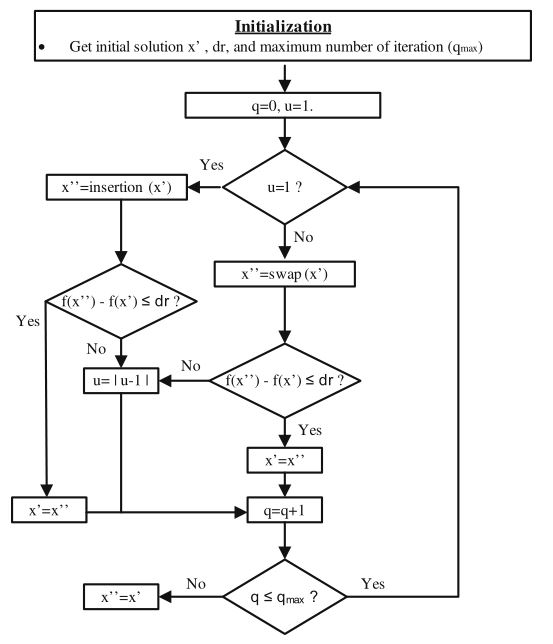
\includegraphics[width = 12cm]{local_search.jpg}
\caption{区域搜索算法流程\label{fig:local_search}}
\end{figure}
\subsubsection{特点分析}
当调度目标函数式多目标的时候,解空间的维度加大,光用区域搜索的方法很容易陷入局部最优,而变动邻域搜索则可通过扰动来使之跳出局部最优。虽然这个方法在解决多目标优化问题的时候效果较好,然而随着目标的复杂程度增加,搜索空间大小将呈现指数增长,求解困难增加。可以通过一些方法,如分支定界或有限差异搜寻等提高搜索质量。另外,有多目标的问题,可以通过神经网络的方法来得到各目标间的权衡系数,以提高目标函数质量。
\subsection{PSO}
\subsubsection{补充概念}
粒子群优化算法(PSO)是一种基于进化计算的随机优化技术,它将搜索空间中的解看作``粒子'',所有粒子都有其由固定函数计算得到的固定值,同时也有其引导飞行的速度。粒子的速度和位置是该方法主要考虑的方面,这是一种形象的利用历史数据作为合理预测的方法,为描述其生成方程,需如下定义:

\vspace{1em}	
\begin{tabular}{ll}	
$i$ & 第$i$个粒子。\\
$X_{i,t}$ & 在迭代$t$中的第$i$个粒子的位置。\\
$V_{i,t}$& 在迭代$t$中的第$i$个粒子的速度。\\
$P_i$&粒子$i$在先前的最好位置。$P_g$为所有粒子中的最好位置\\
$w$&为惯性权重,以平衡局部即全局粒子群的利用。\\
$C_1,C_2$& 在搜寻过程中,控制粒子位置的线性因子。
\end{tabular}
\subsubsection{算法步骤及简单说明}
PSO 方法是通过粒子的位置和速度来执行搜索过程,需要用到如下迭代公式:
\begin{align}
V_{i,t+1} &= wV_{i,t} + Rand C_1(P_i - X_{i,t}) + rand C_2 (P_g - X_{i,t})\label{equ:1}\\
X_{i,t+1} &= X_{i,t} + V_{i,t+1}\label{equ:2}
\end{align}

\eqref{equ:1}为粒子速度迭代式,式中$Rand,rand$皆为区间在$[0,1]$的随机变量。其中第1部分为惯性部分,是粒子前一个阶段的,第2部分为``认知''部分,表示为粒子的``思考'',其自身因素为主,第3部分为``社会化''部分,是由群体因素为主,这样的迭代关系是比较形象的。\eqref{equ:2}为粒子的位置迭代式。由此,可得PSO 的算法步骤:

\begin{asparaenum}
\renewcommand{\labelenumi}{\heiti 步骤\theenumi~}
\item 在一个D维问题空间内初始化一定数量的粒子的速度和位置。
\item 置$P_i$为当前位置,$P_g$为当前的最好位置。
\item 用\eqref{equ:1}和(\ref{equ:2})更新粒子的速度和位置。
\item 计算所有粒子的目标值。
\item 对于每个粒子,如果当前值优于各自的$P_i$,则更新$P_i$为较优值。
\item 同样的更新$P_g$
\item 如果遇到了终止信号,则输出$P_g$以及目标值,否则执行\Step3。
\end{asparaenum}

\subsubsection{特点分析}
PSO 技术只需初级和简单数学操作即可完成,通过粒子的速度和位置两个部分,形象了搜索过程,能较快达到近似最优解,所需时间和成本都较低,能够较好处理目标很多的柔性流水车间调度,然而其能处理的问题规模较小。对于能拆分成小型问题的中大型问题,此方法就很有优势。另一个问题就是迭代式的收敛性,收敛速度决定了计算速度。
\section{方法比较}
通过上述3个算法的特点分析,我们得到了它们的特点,现在需要分析其适用情况,通过比较来启发本课题的研究。

FBFS 算法的特点是将作业按簇分成批次,可以有效减少作业簇准备时间,适合多品种的生产调度,这是直接从调度本身入手的,可操作性很大,而且较符合实用情况,虽然有其不完善,但改善比较容易。VNS 和PSO 都是解的搜索方法,理论性较强,可以将两者结合实用,比如在VNS 随机下一个邻域的的阶段可以通过PSO 来确定下一个搜索方向,发货两者的优势。只是仅从目标函数的解空间搜索,获得的结果可能会在实用中出现相关问题,需要进一步通过实践研究。

\section{小结}
本章首先给出了调度问题的确定型和随机型模型的一般框架和概念,是深入研究本课题的基础,框架中的内容需要根据实际情况作相应的修改和拓展。之后本文列举了3个有关多品种、多目标的调度算法,其中FBFS 直接从调度本身入手,而VNS 和PSO 则从解的搜索入手。FBFS 算法的特点是将作业按簇分成批次,可以有效减少作业簇准备时间,适合多品种的生产调度,然而该方法只按优先级排序作业,按批次的特点安排生产,可能会导致部分作业滞后完成而部分作业却提前完成。这个方面可以通过例如滚动时域的方法将其改善。VNS 可通过扰动来使之跳出局部最优,虽然这个方法在解决多目标优化问题的时候效果较好,然而随着目标的复杂程度增加,搜索空间大小将呈现指数增长,求解困难增加。可以通过一些方法,如分支定界或有限差异搜寻等提高搜索质量。同时,也可通过神经网络的方法来得到各目标间的权衡系数,以提高目标函数质量。PSO 技术只需初级和简单数学操作即可完成,通过粒子的速度和位置两个部分,形象了搜索过程,能较快达到近似最优解,所需时间和成本都较低,能够较好处理目标很多的柔性流水车间调度,然而其能处理的问题规模较小。对于能拆分成小型问题的中大型问题,此方法就很有优势。此外要关注起收敛速度。